%                                                                 aa.dem
% AA vers. 8.2, LaTeX class for Astronomy & Astrophysics
% demonstration file
%                                                       (c) EDP Sciences
%-----------------------------------------------------------------------
%
%\documentclass[referee]{aa} % for a referee version
%\documentclass[onecolumn]{aa} % for a paper on 1 column  
%\documentclass[longauth]{aa} % for the long lists of affiliations 
%\documentclass[rnote]{aa} % for the research notes
%\documentclass[letter]{aa} % for the letters 
%\documentclass[bibyear]{aa} % if the references are not structured 
% according to the author-year natbib style

%
\documentclass{aa}  
%
%

\usepackage{graphicx}
%%%%%%%%%%%%%%%%%%%%%%%%%%%%%%%%%%%%%%%%
\usepackage{txfonts}
%%%%%%%%%%%%%%%%%%%%%%%%%%%%%%%%%%%%%%%%
\usepackage{hyperref}
\pdfoutput=1
\usepackage{amsfonts}
\usepackage{amsmath}
\usepackage{amssymb}
\usepackage{xcolor}
\usepackage{enumitem}
\usepackage{graphicx}
\usepackage{gensymb}
\usepackage{fancyhdr}
\usepackage{times}
\usepackage{ulem}
%\usepackage{caption}
\usepackage{subcaption} 
\usepackage{float} 
\usepackage{color}
\usepackage{booktabs}
\usepackage{lscape}
\usepackage{xspace}
 
%\usepackage[options]{nohyperref}

\definecolor{purple}{RGB}{76, 0,153}
\newcommand{\ch}[1]{{\color{purple}{#1}}}
\newcommand{\preliminary}[1]{\textcolor{orange}{#1}}
\newcommand{\TT}[1]{{\color{purple}{TT: #1}}}

\newcommand{\dd}{{\rm d}}
\newcommand{\diff}{{\rm d}}

\newcommand{\br}[1]{\left( #1 \right)}
\newcommand{\bc}[1]{\left\{ #1 \right\}}
\newcommand{\eqa}[1]{\begin{align}   #1 \end{align}}

\newcommand{\bb}[1]{\left[ #1 \right]}
\newcommand{\vek}[1]{\mbox{\boldmath $#1$}}

\newcommand{\software}[1]{\texttt{#1}}
\newcommand{\tttp}{$3\times2$pt\xspace}
\newcommand{\kpoff}{\ensuremath{3.1\,\sigma}\xspace}
\newcommand{\kpoffperc}{\preliminary{$8.2 \pm 2.6$\%}\xspace}
\newcommand{\kSeightval}{\preliminary{$0.769^{+0.018}_{-0.015}$}\xspace}
\newcommand{\klogR}{\ensuremath{3.1\pm0.3}\xspace}
\newcommand{\kR}{\ensuremath{23\pm6}\xspace}
\newcommand{\klogS}{\ensuremath{-2.0\pm0.1}\xspace}
\newcommand{\klogSPTE}{\ensuremath{0.08\pm0.2}\xspace}
\newcommand{\klogSPTEsigma}{\ensuremath{1.8\pm0.1\,\sigma}\xspace}

\newcommand{\LCDM}{$\Lambda$CDM\xspace}

\newcommand{\be}{\begin{equation}}  \newcommand{\ee}{\end{equation}}

\usepackage{environ}
\NewEnviron{splitequation}{%
    \begin{equation}\begin{split}
        \BODY
    \end{split}\end{equation}}
    
\begin{document} 

   \title{KiDS-1000 Cosmology: Multi-probe weak gravitational lensing and spectroscopic galaxy clustering constraints}

   \author{Catherine Heymans \inst{1,2}\thanks{Catherine Heymans: heymans@roe.ac.uk} 
   \and Tilman Tr\"oster\inst{1}\thanks{Tilman Tr\"oster: ttr@roe.ac.uk} 
   \and Marika Asgari\inst{1} 
   \and Chris Blake\inst{3}
   \and Hendrik Hildebrandt\inst{2}
   \and Benjamin Joachimi\inst{4}
   \and Chieh-An Lin\inst{1}
   \and Ariel~G.~S\'anchez\inst{5}
   \and Jan Luca van den Busch\inst{2}
   \and Angus~H.~Wright\inst{2}
   \and Maciej Bilicki\inst{6}
   \and Andrej Dvornik\inst{2}
   \and Thomas Erben\inst{7}
   \and Benjamin Giblin\inst{1}
   \and Arun Kannawadi\inst{8,9}	
   \and Fabian K\"ohlinger\inst{2}
   \and Konrad Kuijken\inst{10}
   \and Peter Schneider \inst{7}
   \and the KiDS Collaboration
          }
\institute{Institute for Astronomy, University of Edinburgh, Royal Observatory, Blackford Hill, Edinburgh, EH9 3HJ, UK 
   \and
   Ruhr-Universit{\"a}t Bochum, Astronomisches Institut, German Centre for Cosmological Lensing (GCCL), Universit{\"a}tsstr.  150, 44801, Bochum, Germany
   \and 
   Centre for Astrophysics \& Supercomputing, Swinburne University of Technology, P.O. Box 218, Hawthorn, VIC 3122, Australia
   \and
   Department of Physics and Astronomy, University College London, Gower Street, London WC1E 6BT, UK
   \and
   Max-Planck-Institut f\"ur extraterrestrische Physik, Postfach 1312, Giessenbachstrasse 1, D-85741 Garching, Germany
   \and 
   Center for Theoretical Physics, Polish Academy of Sciences, al. Lotnik\'{o}w 32/46, 02-668, Warsaw, Poland
   \and
   Argelander-Institut f. Astronomie, Univ. Bonn, Auf dem Huegel 71, D-53121 Bonn, Germany
    \and
   Department of Astrophysical Sciences, Princeton University, 4 Ivy Lane, Princeton, NJ 08544, USA
    \and
   Leiden Observatory, Leiden University, Niels Bohrweg 2, 2333 CA Leiden, the Netherlands
   }
 %  \date{Received September 15, 1996; accepted March 16, 1997}

% 5 {} token are mandatory
 
  \abstract{We present a joint cosmological analysis of weak gravitational lensing observations from the Kilo-Degree Survey (KiDS-1000), with redshift-space galaxy clustering observations from the Baryon Oscillation Spectroscopic Survey (BOSS), and galaxy-galaxy lensing observations from the overlap between KiDS-1000, BOSS and the spectroscopic 2-degree Field Lensing Survey (2dFLenS).  This combination of large-scale structure probes breaks the degeneracies between cosmological parameters for individual probes, resulting in a constraint on the structure growth parameter $S_8=\sigma_8 \sqrt{\Omega_{\rm m}/0.3} =$ \kSeightval, that has the same precision as that reported by the full-sky cosmic microwave background observations from {\it Planck}.   The recovered $S_8$ amplitude is low, however, by \kpoffperc relative to {\it Planck}.   This result builds from a series of KiDS-1000 analyses where we validate our methodology with variable depth mock galaxy surveys,  our lensing calibration with image simulations and null-tests, and our optical-to-near-infrared redshift calibration with multi-band mock catalogues and a spectroscopic-photometric clustering analysis.   The systematic uncertainties identified by these analyses are folded through as nuisance parameters in our cosmological analysis.  Inspecting the offset between the marginalised posterior distributions, we find that the $S_8$-difference with {\it Planck} is driven by a tension in the matter fluctuation amplitude parameter, $\sigma_8$.   
We quantify the level of agreement between the CMB and large-scale structure constraints using a series of different metrics, finding differences with a significance ranging between $\sim 2\sigma$ and $\sim 3\sigma$. \preliminary{Final MAP optimisation runs are almost complete - results in this colour will be updated after the weekend.}}

 \keywords{gravitational lensing: weak, methods: data analysis, methods: statistical, surveys, cosmology: observations}

   \titlerunning{KiDS-1000: 3x2pt}
   \authorrunning{Heymans, Tr\"oster \& the KiDS Collaboration et al.}
   \maketitle
%
%________________________________________________________________
\section{Introduction}
\label{sec:intro}

Observations of the cosmic microwave background (CMB) have delivered high-precision
constraints for the cosmological parameters of the flat, cold dark
matter and cosmological constant model of the Universe
\citep[$\Lambda$CDM,][]{planck/etal:2018}.  With only six free
parameters, this flat $\Lambda$CDM model provides an exquisite fit to observations of
the anisotropies in the CMB.    The same model predicts a range of
different observables in the present day Universe, including the cosmic expansion rate \citep{weinberg/1972}, and the
distribution of, and gravitational lensing by, large-scale
structures \citep{peebles/1980,bartelmann/schneider:2001,eisenstein/etal:2005}.  
In most cases there
is agreement between the measured cosmological parameters of the flat $\Lambda$CDM model, when comparing those
constrained at the CMB epoch with those constrained through a variety of
lower-redshift probes \citep[see the discussion in][and references
therein]{planck/etal:2018}.   Recent improvements in the statistical
precision of the lower-redshift probes have,
however, revealed some statistically significant differences.  Most
notably a $4.4\sigma$ difference in the value of the Hubble constant,
$H_0$, has been reported using distance ladder estimates in \citet{riess/etal:2019}.  If this difference cannot be
attributed to systematic errors in either, or both, experiment, this result
suggests that the flat $\Lambda$CDM model is incomplete.

Many
extensions have been proposed to reconcile the observed differences between
high- and low-redshift probes \citep[see for
example][]{riess/etal:2016,poulin/etal:2018,divalentino/etal:2020}.  All, however, require
additional components
to the cosmological model that move it even further away from the
standard model of particle physics, a model that already struggles to motivate
the existence of cold dark matter and a cosmological constant.  
As the statistical power of the observations continues to improve, focus has moved to establishing
a full understanding of all systematic errors, and the development of mitigation approaches, 
in preparation for the high-precision `full-sky' imaging and spectroscopic
cosmology surveys of the 2020's \citep[{\it Euclid},][]{laureijs/etal:2011,lsst/etal:2009,DESI/etal:2016}.

In this analysis we present a multi-probe `same-sky' analysis of the
evolution of large-scale structures, using imaging and spectroscopic surveys.
Our first observable is the weak gravitational lensing of background
galaxies by foreground large-scale
structures, 
known as `{\it cosmic shear}'.    Our second
observable is the {\it anisotropic clustering of galaxies} within these
large-scale structures, combining measurements of both redshift-space
distortions and baryon acoustic
oscillations.   Our third observable is the weak gravitational lensing of background
galaxies by foreground galaxies, known as
`{\it galaxy-galaxy lensing}'.   As these three sets of two-point
statistics are analysed simultaneously, this combination of probes
is usually referred to as a `\tttp' analysis. 

Each observable in our multi-probe analysis is subject to systematic
uncertainties.  For a cosmic shear analysis, the observable is a
combination of the true cosmological signal with a low-level signal
arising from the intrinsic alignment of galaxies, as well as potential residual
correlations in the data induced by the atmosphere, telescope and
camera.   The signal can also be scaled by both shear
 and photometric redshift measurement calibration errors
 \citep[see][and references therein]{mandelbaum:2018}.   For a galaxy
   clustering analysis, the observable is the true
   cosmological signal modulated by an uncertain, non-linear and
   evolving, galaxy bias function.  This function maps how
   the galaxies trace the
   underlying total matter distribution \citep[see][and references
   therein]{desjacques/etal:2018}. 
   The cosmological clustering
   also needs to be accurately distinguished from artificial clustering in the galaxy sample,
   arising from potentially uncharacterised inhomogeneities in the target selection \citep[see for example][]{ross/etal:2012}. 
   Finally, the galaxy-galaxy
   lensing analysis is subject to the systematics that impact both the
   cosmic shear and clustering analyses.

   When analysing these
   observables in combination
   the different astrophysical and systematic dependencies allow for some degree of
   self-calibration \citep{bernstein/jain:2004, hu/jain:2004,
     bernstein:2009,joachimi/bridle:2010}.  `Same-sky'
   surveys, in which imaging for weak lensing observables overlaps with
   spectroscopy for anisotropic galaxy clustering measurements,
   also allows for their cross-correlation.  Such a survey design therefore
   presents a robust
   cosmological tool that can calibrate and mitigate systematic and astrophysical
   uncertainties through a series of nuisance parameters.   In
   addition to enhanced control over systematics, this combination of probes
   breaks cosmological parameter degeneracies from each individual
   probe. 
   For a flat $\Lambda$CDM model
   this leads to significantly tighter constraints on the matter fluctuation amplitude 
   parameter, $\sigma_8$, and the matter density parameter, $\Omega_{\rm m}$, whilst also decreasing the
   uncertainty on the recovered dark energy equation of state
   parameter in extended cosmology scenarios \citep{hu/jain:2004,gaztanaga/etal:2012}.
   
   Three variants of a joint `\tttp' analysis have been
   conducted to date.  \citet{vanuitert/etal:2018} present a joint power-spectrum
   analysis of the Kilo-Degree Survey \citep[KiDS,][]{kuijken/etal:2015} with
   the Galaxy And Mass Assembly survey
   \citep[GAMA,][]{liske/etal:2015}, incorporating projected
   angular clustering measurements.   \citet{joudaki/etal:2018}
   present a joint analysis of KiDS with the
   2-degree Field Lensing Survey \citep[2dFLenS,][]{blake/etal:2016}
   and the overlapping area in the Baryon Oscillation Spectroscopic Survey \citep[BOSS,][]{alam/etal:2015}, incorporating
   redshift-space clustering measurements.  \citet{abbott/etal:2018}
   present a joint real-space lensing-clustering analysis of the Dark
   Energy Survey \citep[DES,][]{drlicawagner/etal:2018}, using a high-quality
   photometric redshift sample of luminous red galaxies for their projected
   angular clustering measurements.  
   In all three cases a
   linear galaxy bias model was adopted. 
   
   In this analysis we enhance and build upon the advances of previous `\tttp' studies.   We analyse the most recent KiDS data release \citep[KiDS-1000,][]{kuijken/etal:2019}, more than doubling the
   survey area from previous KiDS studies.   We utilise the full BOSS
   area and the `full-shape' anisotropic clustering measurements of \citet{sanchez/etal:2017},
   incorporating information from both redshift-space distortions
   and the baryon acoustic oscillation as our galaxy clustering probe.   We adopt a non-linear
   evolving galaxy bias model, derived from renormalised perturbation theory
   \citep{crocce/scoccimarro:2006, chan/etal:2012}.  
   We maximise the signal-to-noise in our 
   KiDS-BOSS galaxy-galaxy lensing analysis, 
   by including additional overlapping spectroscopy of BOSS-like galaxies from 2dFLenS.

This paper is part of the KiDS-1000 series.  The KiDS-1000 photometry and imaging is presented in \citet{kuijken/etal:2019}.  The core weak lensing data products are presented and validated in \citet[shear measurements,][]{giblin/etal:inprep},  and  \citet[redshift measurements,][]{hildebrandt/etal:inprep}.   \citet{asgari/etal:inprep} conduct the cosmic shear analysis using a range of different two-point statistics, and \citet{joachimi/etal:inprep} detail the methodology behind our `\tttp'  
   analysis, with a particular focus on pipeline validation and accurate covariance matrices.   In this analysis we constrain the cosmological parameters of the flat $\Lambda$CDM model.   A range of different extensions to the $\Lambda$CDM model are considered in \citet{troester/etal:inprep}, including varying dark energy, neutrino mass, spatial curvature and various modified gravity scenarios \citep{bose/etal:2020}.
   This paper is organised as follows.   We review the data and provide a concise summary of the findings of the KiDS-1000 series of papers in Section~\ref{sec:data}.   
 We present our joint cosmological constraints in Section~\ref{sec:results}, and conclude in Section~\ref{sec:conc}.  Appendices tabulate the galaxy properties (\ref{app:properties}), the adopted cosmological parameter priors (\ref{app:priors}),  and the cosmological parameter constraints (\ref{app:parameter-constraints}).   They also discuss a series of sensitivity tests (\ref{app:sensitivity}), the redundancy, validation and software review for our pipeline (\ref{app:codereview}), and detail the minor analysis additions that were included after the analysis was formally unblinded (\ref{app:unblinding}).


   











   
\section{Data}
\label{sec:data}

\subsection{Surveys:  KiDS, BOSS and 2dFLenS}
\label{sec:surveys}
Summary of \citet{kuijken/etal:2019},  \citet{blake/etal:2016}, \citet{alam/etal:2015}

\subsection{Cosmic Shear}
\label{sec:cosmic_shear}
Summary of \citet{asgari/etal:inprep}

\begin{figure}
        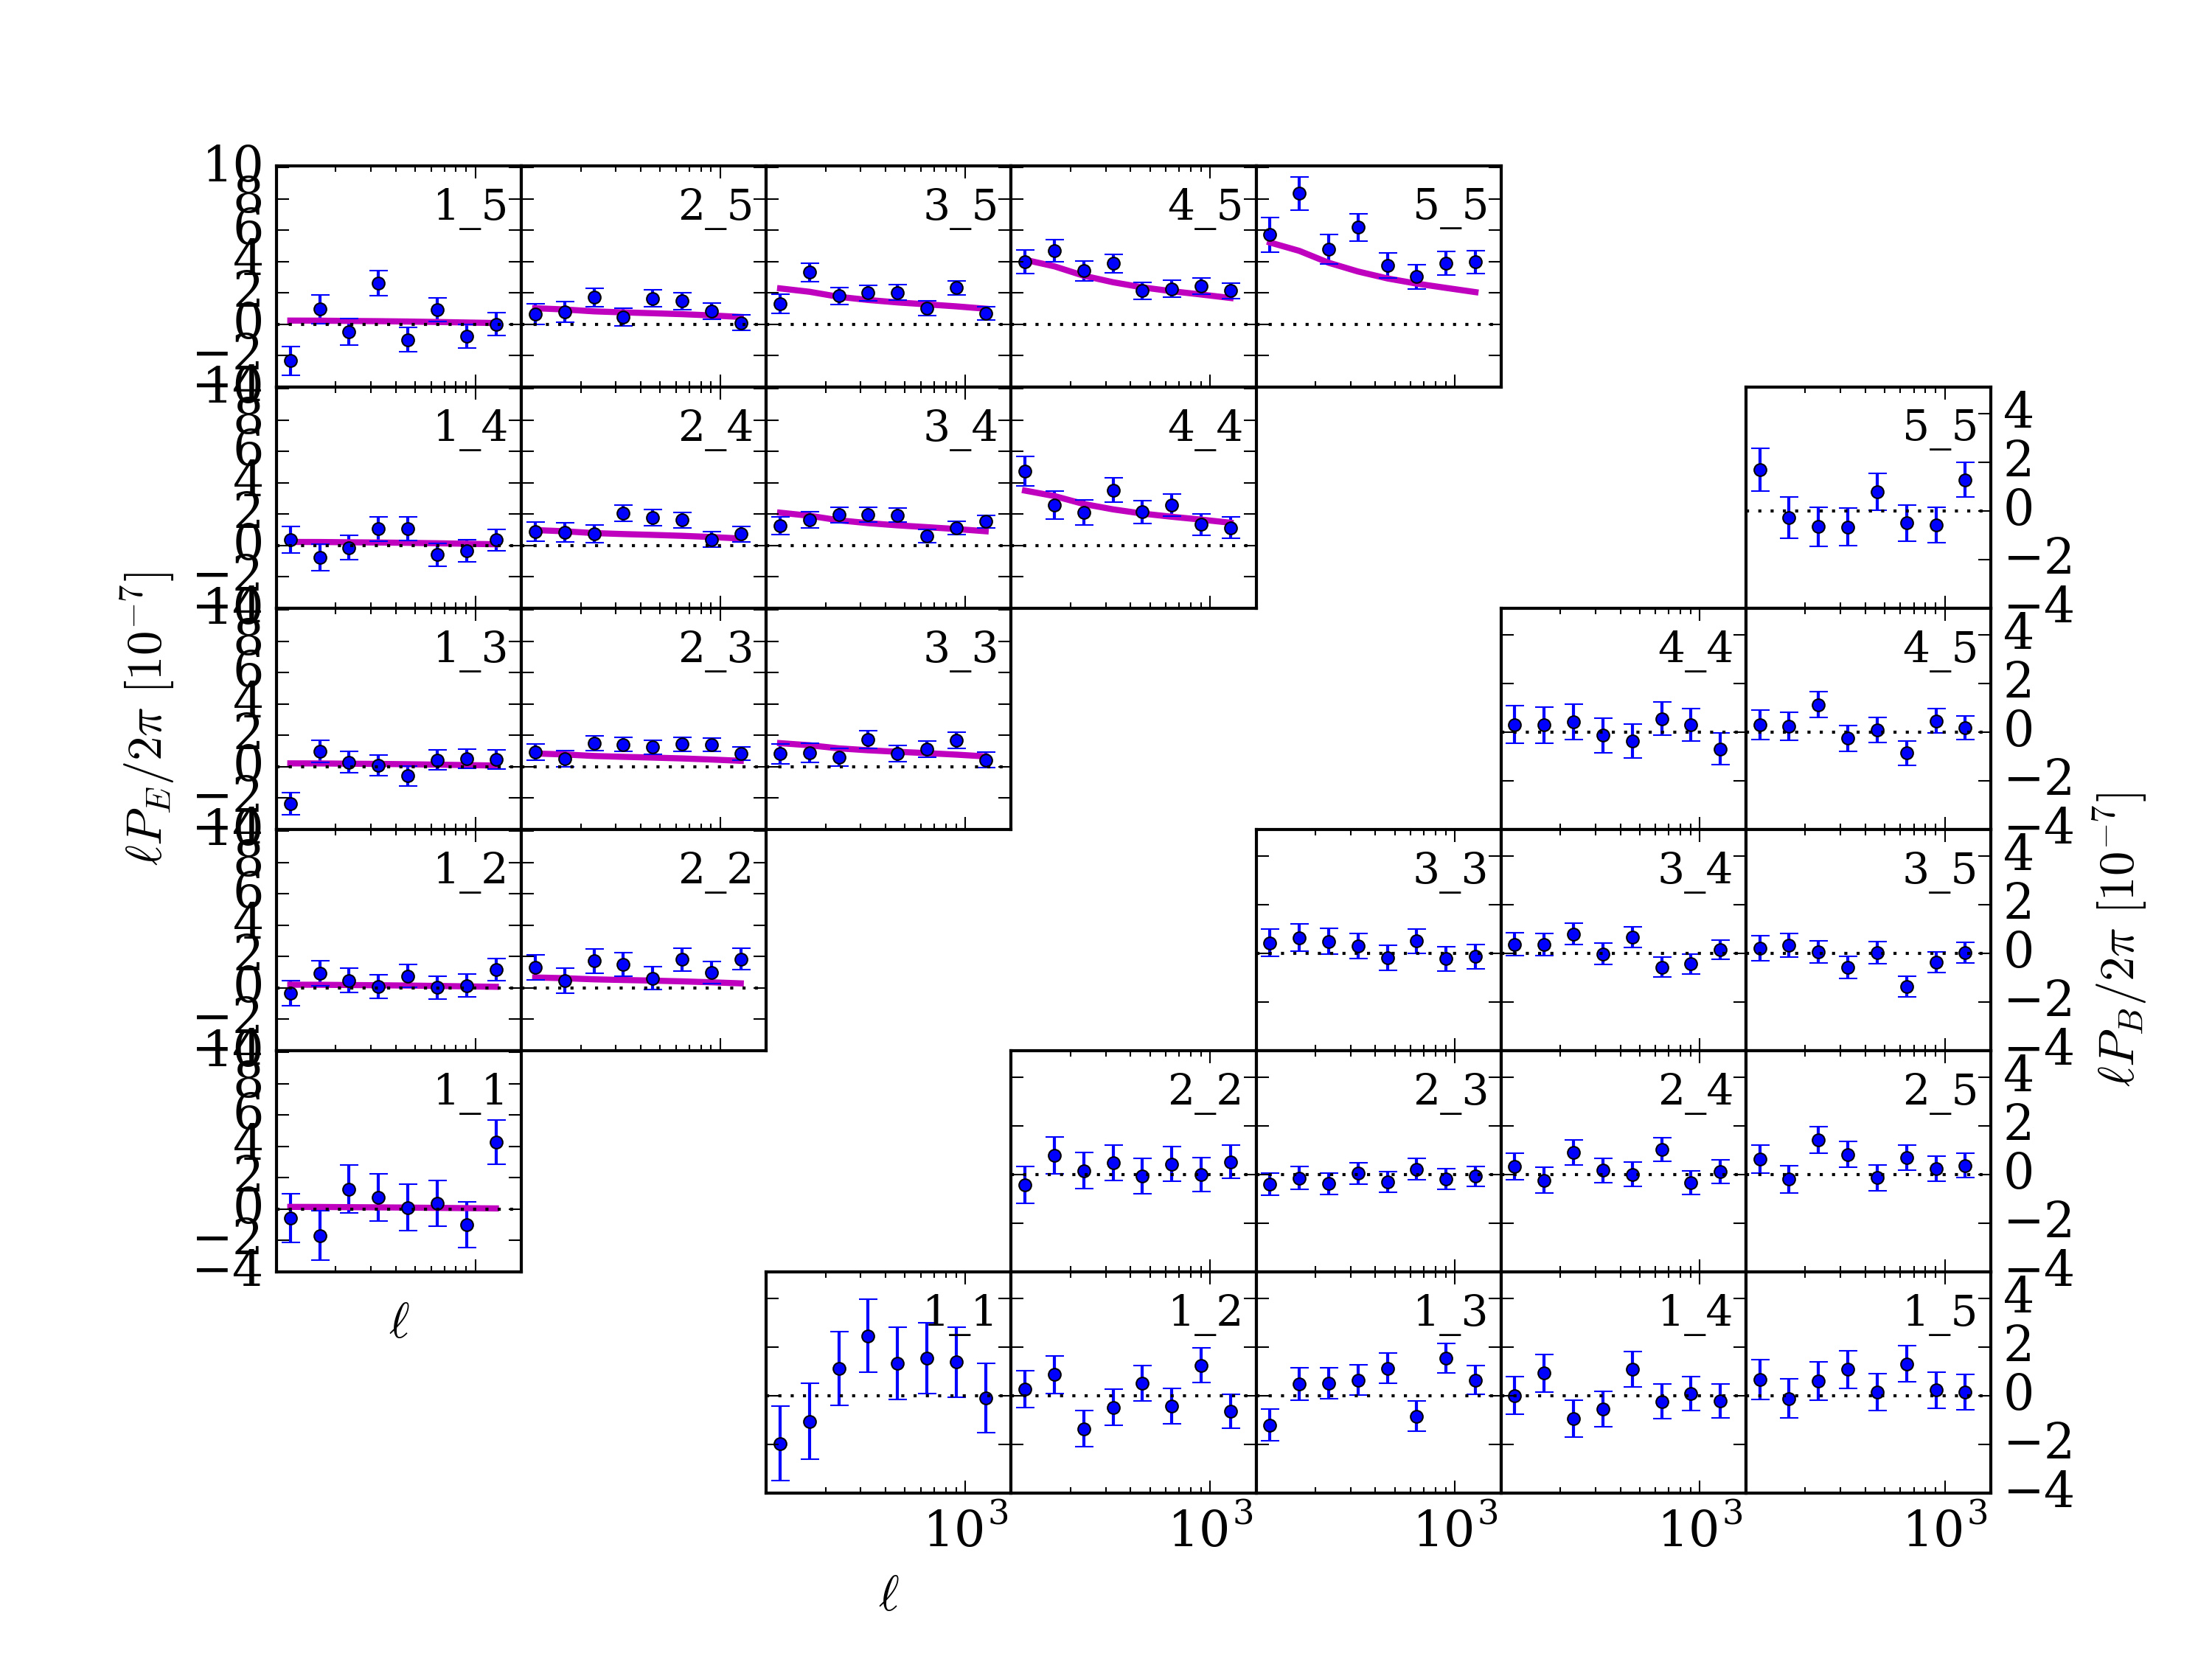
\includegraphics[width=\columnwidth]{Data_Plots/Pkk/Pkk_K1000_2Dbins_v2_goldclasses_Flag_SOM_Fid.png}
        \caption{To do }
        \label{fig:Pkk}
\end{figure}

\subsection{Galaxy-Galaxy Lensing}
\label{sec:GGL}
Summary of Blake et al?

\subsection{Anisotropic Galaxy Clustering}
\label{sec:clustering}
Summary of \citet{sanchez/etal:2017}

\subsection{Covariance}
\label{sec:Cov}
Summary of \citet{joachimi/etal:inprep}


\section{Results}
\label{sec:results}
We present our joint multi-probe constraints on the cosmological parameters of the flat $\Lambda$CDM parameters in Fig.~\ref{fig:cosmology-params}, showing the marginalised posterior distributions for $\sigma_8$, $\Omega_{\rm m}$ and $h$.   Reporting the best-fit MAP with PJ-HPD values for the two parameters that we are most sensitive to, we find (Blind A)
\eqa{
\sigma_8 &= 0.781^{+0.025}_{-0.019} \\ \nonumber
\Omega_{\rm m} &= 0.321^{+0.016}_{-0.010} \\ \nonumber
S_8 &= 0.791^{+0.020}_{-0.012} \, ,
}
where the BOSS galaxy clustering constraints (GC: shown blue), break the $\sigma_8-\Omega_{\rm m}$ degeneracy in the KiDS-1000 cosmic shear constraints (CS: shown pink), resulting in tight constraints on $\sigma_8$ in the combined $3\times2{\rm pt}$ analysis (shown red).   Our constraints can be compared to the marginalised posterior distributions from Planck (shown green), which we discuss in more detail in Sect.~\ref{sec:planck_comp}.

Tabulated constraints for the full set of cosmological parameters are presented in Appendix~\ref{app:parameter-constraints}, quoting our fiducial MAP with PJ-HPD credible intervals, along with the standard marginal posterior mode with M-HPD credible intervals.   We note that the standard quoted marginal mode constraint on $S_8$ is $\sim 10\%$ tighter than the MAP constraint.  As discussed in \citet{joachimi/etal:inprep}, however, this estimate can be easily misinterpreted, yielding systematically low values of $S_8$ in mock data analyses.   This now known bias, can be seen in Fig.~\ref{fig:S8comp}, which compares the MAP constraints (solid) with the marginal (dashed).  

\begin{figure}
	\begin{center}
		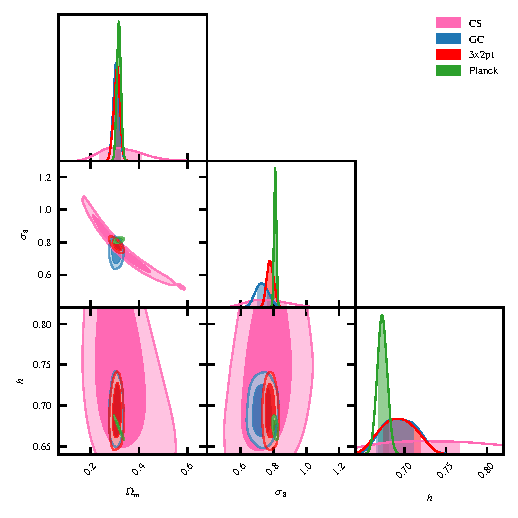
\includegraphics[width=\columnwidth]{Parameter_Plots/cosmology/omegam_sigma8_h_blind_A}
		\caption{Constraints on flat $\Lambda$CDM blind A}
		\label{fig:cosmology-params}
	\end{center}
\end{figure}

We find good agreement between the different probe combinations and single probe $S_8$ constraints, demonstrating internal consistency between the different cosmological probes, in Fig.~\ref{fig:S8comp}.  As forecast by \citet{joachimi/etal:inprep}, the addition of the galaxy-galaxy lensing observable adds very little constraining power, with similar results found for the full $3\times2{\rm pt}$ analysis and the combined cosmic shear and clustering analysis.   This is a result of the significant area of BOSS in comparison to KiDS-1000, and the fact that our lack of an accurate non-linear galaxy bias model prohibits the inclusion of large sections of our galaxy-galaxy lensing data vector, shown in Fig.~\ref{fig:Pgk}.     The addition of the galaxy-galaxy lensing does however serve to moderately tighten constraints on the amplitude of the intrinsic alignment model $A_{\rm IA}$. 

\begin{figure}
	\begin{center}
		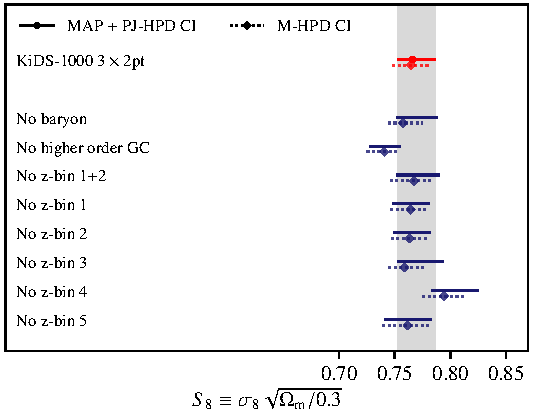
\includegraphics[width=\columnwidth]{Parameter_Plots/systematics/S8_comparison_blindC}
		\caption{Constraints on $S_{8}$ blind C. \TT{Note that the 3x2pt chain has the clustering bug fixed, hence the overall offset.}}
		\label{fig:S8comp}
	\end{center}
\end{figure}

The lower section of Fig.~\ref{fig:S8comp} illustrates the results of a series of sensitivity tests, where we explore how our constraints on $S_8$ change when: we ignore the impact of baryon feedback (the `No baryon' case), fixing $A_{\rm baryon}=3.13$, corresponding to the non-linear matter power spectrum for a dark-matter only cosmology; we limit the analysis to a linear galaxy bias model, setting all higher-order bias terms in Eq.(\ref{eq:pgg}), to zero; when we remove individual tomographic bins from our weak lensing observables.    The only outlier in this series of tests is the linear-bias model, which highlights the importance of accurate non-linear galaxy bias modelling in $3\times2$pt analyses.    This series of tests complements the more detailed KiDS-1000 internal consistency analysis of \citet{asgari/etal:inprep}, and is dissected in Appendix~\ref{app:sensitivity}.

Fig.~\ref{fig:cosmology-params-all} displays the marginalised posterior distributions for an extended set of cosmological parameters.   We find that the constraint on galaxy bias,  $b_1$, in each redshift bin (lower two rows), is more than halved with the addition of the weak lensing data.   This constraint does not arise, however, from the sensitivity of the galaxy-galaxy lensing observable to galaxy bias.  Instead, in this analysis, it is a result of the degeneracy breaking in the $\sigma_8-\Omega_{\rm m}$ plane, tightening constraints in $\sigma_8$ which, for galaxy clustering, is fully degenerate with galaxy bias.  The improved constraints on galaxy bias do not, however, fold through to improved constraints on $h$, which the weak lensing data adds very little information to.

For the majority of the cosmological parameters shown in Fig.~\ref{fig:cosmology-params-all}, the constraints are uninformed by our choice of prior.  The three key exceptions are the spectral index, $n_{\rm s}$, the Hubble parameter, $h$, and the baryon feedback amplitude, $A_{\rm baryon}$.  As noted by \citet{troester/etal:2020}, the BOSS galaxy clustering constraints favour a low value for $n_{\rm s}$, where they find $n_{\rm s} = 0.815 \pm 0.085$.  They conclude that this preference is primarily driven by the amplitude of the large scale clustering signal with $s > 100 \, h^{-1}\, {\rm Mpc}$.  As spurious excess power in this regime could plausibly arise from variations in the stellar density impacting the BOSS galaxy selection function \citep{ross/etal:2017}, we chose to impose an informative prior for $n_{\rm s}$, as listed in Table~\ref{tab:priors}.   This prior does not degrade the overall goodness of fit to the galaxy clustering measurements, and is no more informative than the $n_{\rm s}$ priors that are typically used in weak lensing and clustering analyses \citep[see for example][]{sanchez/etal:2017,abbott/etal:2018}.  We do recognise, however, that this choice of prior serves to reduce the BOSS-only error on $\Omega_{\rm m}$ by roughly a third (see Appendix~\ref{app:priors}).   We note that the galaxy clustering preference for low $n_{\rm s}$ also leads to the joint $3\times2{\rm pt}$ constraint favouring the dark-matter only value for the baryon feedback amplitude $A_{\rm baryon}$.   This preference is not significant however, with all values of $A_{\rm baryon}$ within the prior region, compatible at the $<2 \sigma$ level.   BOSS also provides reasonable constraints on $h$, with our $1\sigma$ constraints on $h$ lying within the $h$-prior.   As the marginal probability at the lower prior edge exceeds 20\% of the peak probability, however, we consider this parameter unconstrained by our analysis.

\begin{figure*}
	\begin{center}
		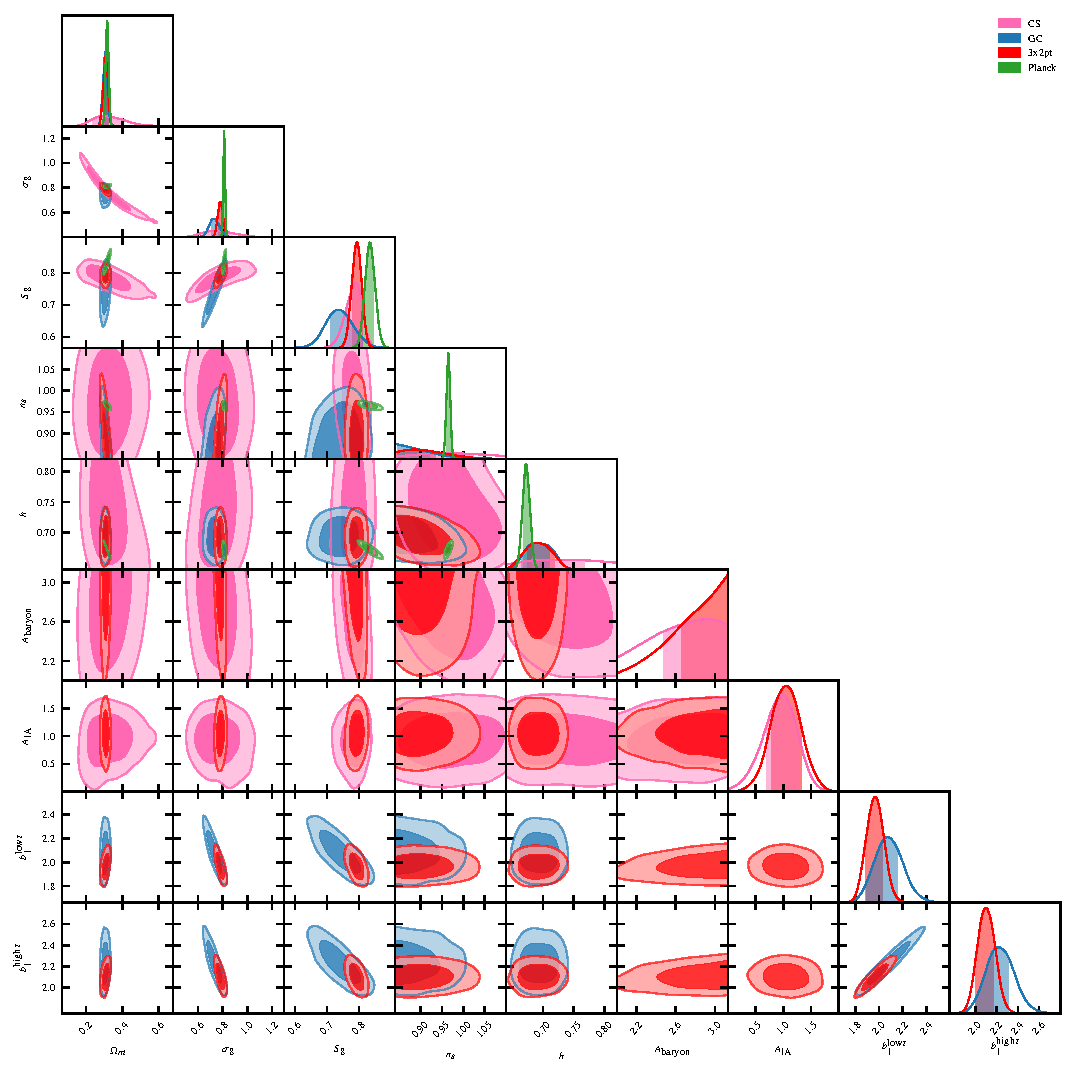
\includegraphics[width=\textwidth]{Parameter_Plots/cosmology/omegam_sigma8_s8_ns_h_a_baryon_a_ia_b1l_b1h_blind_A}
		\caption{Constraints blind A}
		\label{fig:cosmology-params-all}
	\end{center}
\end{figure*}

Table~\ref{tab:goodness-of-fit} records the goodness of fit for each component in our $3\times2$pt analysis.  The effective number of degrees of freedom (DoF) are calculated using the estimator described in section 6.3 of \citet{joachimi/etal:inprep}.   The goodness of fit in all cases is acceptable, but only just.    We are unconcerned by these results, however, given the cosmic shear analysis of \citet{asgari/etal:inprep}, where a different choice in the cosmic shear two-point statistic results in an excellent goodness of fit, with no significant changes in the inferred cosmological parameters.    As such, we could be subject to an unlucky noise fluctuation that particularly impacts the band power estimator in Eq.(\ref{eq:cl_cosmicshear}.  Cautiously inspecting Fig.~\ref{fig:Pkk}, as `$\chi$-by-eye' is particularly dangerous with correlated data points, we nevertheless note a handful of outlying points, for example the low$\ell$-scales in the fifth tomographic bin.   We also note that \citet{giblin/etal:inprep} document a significant but low-level PSF residual systematic in the KiDS-1000 fourth and fifth tomographic bins that was shown to reduce the overall goodness of fit in a cosmic shear analysis, but not bias the recovered cosmological parameters \citep[see also the discussion in][]{amara/refregier:2008}.  Future work to remove these low-level residual distortions are therefore expected to improve the goodness of fit further.

\begin{table}
	\begin{center}
		\caption{Goodness of fit for blind A}
		\label{tab:goodness-of-fit}
\begin{tabular}{lrcl}
    \toprule
    Probe             & $\chi^2$       & DoF       & $p$-value   \\
    \midrule
	CS               & $< 156.3$ & $120-4.5$ & 0.007 \\
	GC               & $< 169.5$ & $168-13$ & 0.202 \\
	CS+GGL           & $187.0$ & $142-7$ & 0.002 \\
	$3\times2$pt            & $367.8$ & $310-20$ & 0.001 \\

    \bottomrule
\end{tabular}
	\end{center}
\end{table}


\subsection{Comparison with Planck}
\label{sec:planck_comp}
This section we will write post-blinding, as until we know which blind it is, it is hard to write.   The short version is A: no tension,  B: oodles of tension,  C: hum.....




\section{Conclusions}
\label{sec:conc}
In this analysis we have presented constraints on the flat $\Lambda$CDM cosmological model by combining observations of gravitational lensing and galaxy clustering to directly probe the evolution and distribution of the large-scale structures in the Universe.    Our survey of the $z \lesssim 1$ low-redshift Universe finds a matter distribution that is less clustered, compared to predictions from the best-fitting $\Lambda$CDM model to early-Universe CMB observations \citep{planck/etal:2018}.  This tendency for low-redshift probes to favour a smoother matter distribution compared to the CMB expectation has persisted since the first large-scale weak lensing survey \citep[CFHTLenS,][]{heymans/etal:2013}, but the significance of this effect has always been tantalisingly around, or below, the $\sim\! 3\,\sigma$ level.   It is therefore unclear if these differences are merely a statistical fluctuation, unaccounted for systematic errors, or a sign of interesting new physics.

Our new result does not lead to a resolution in the matter of statistical fluctuations, finding a \kpoff offset in the structure growth parameter $S_8 = \sigma_8 \sqrt{\Omega_{\rm m}/0.3}$ with $S_8=$\kSeightval.  Comparing the marginal $S_8$ constraints, we find $S_8$ to be \kpoffperc lower than the CMB constraint from \citet{planck/etal:2018}.   For a series of `tension' metrics that quantify differences in terms of the full posterior distributions, we find that the KiDS-1000 and {\it Planck} results agree at the $\sim\! 2\,\sigma$ level.   Through our series of image simulation analyses \citep{kannawadi/etal:2019}, catalogue null-tests \citep{giblin/etal:inprep}, variable depth mock galaxy survey analyses \citep{joachimi/etal:inprep}, optical-to-near-infrared photometric-spectroscopic redshift calibration, validated with mocks \citep{wright/etal:2020, vandenbusch/etal:2020,hildebrandt/etal:inprep}, internal consistency tests \citep[][Fig.~\ref{fig:cosmology-params-all} and Appendix~\ref{app:sensitivity}]{asgari/etal:inprep}, and marginalisation over a series of nuisance parameters that encompass our theoretical and calibration uncertainties (Appendix~\ref{app:priors}),  we argue that we have, however, addressed the question of \tttp systematic errors, robustly assessing and accounting for all sources of systematics that are known about in the literature.    

The KiDS-1000 cosmic shear constraints are highly complementary to the BOSS galaxy clustering constraints, leading to tight constraints in our joint \tttp analysis that are more than twice as constraining for the matter fluctuation amplitude parameter, $\sigma_8 = 0.760^{+0.021}_{-0.023}$, compared to previous \tttp analyses.    In the future, analysis of the clustering and galaxy-galaxy lensing of photometric samples with very accurate photometric redshifts \citep[see for example][]{vakili/etal:2019}, presents an opportunity for a future alternative KiDS-only \tttp photometric analysis, similar to the approach taken in \citet{abbott/etal:2018}.

In the next few years, two weak lensing surveys will see first light, with the launch of the {\it Euclid} satellite and the opening of the Vera~C.~Rubin Observatory.   These observatories will build the first two `full-sky' weak lensing surveys, which are highly complementary in terms of their differing strengths in depth and spatial resolution\footnote{The space-based Nancy Grace Roman Telescope is currently scheduled for launch in 2025 \citep{akeson/etal:2019}, joining {\it Euclid} and {\it Rubin} as an optimal weak lensing observatory for the future.}.  Combined with complementary overlapping redshift spectroscopy from DESI, 4MOST and {\it Euclid}, the multi-probe weak lensing and spectroscopic galaxy clustering methodology, which we have implemented in this analysis, provides a promising route forward for these next generation surveys.   We view this \tttp approach as just the start of the story, however, looking forward to a future combined analysis of weak lensing and galaxy clustering with both photometric and spectroscopic lenses, a combination which we call a `$6\times2$pt' approach \citep{bernstein:2009}.    This would allow for the optimal combination of information from the clustering cross-correlation of spectroscopic and photometric galaxies \citep{newman:2008}, an observable that we currently only use as an independent tool to validate our photometric redshift calibration \citep{hildebrandt/etal:inprep}.      Developments in the area of highly non-linear galaxy bias, baryon feedback and intrinsic alignment modelling, along with a sufficiently flexible but tractable redshift distribution model and an accurate `$6\times2$pt' covariance estimate, will all be required in order to realise this long-term goal.   The effort will, however, be worthwhile allowing for the implementation of arguably the most robust methodology available to mitigate systematic errors, whilst simultaneously enhancing cosmological parameter constraints.

The ESO-KiDS public survey completed observations in July 2019, spanning $1350\,\mathrm{deg}^{2}$.   We therefore look forward to the fifth and final KiDS data release, `KiDS-Legacy', along with new results from the concurrent `Stage-III' surveys, DES and HSC, whilst the community prepares for the next exciting chapter of `full-sky' weak lensing surveys.  

\begin{acknowledgements}
We are completely indebted to Eric Tittley at the IfA for going well beyond the call of duty to save the KiDS-1000 data products after an explosion in our server room destroyed the RAID.   We also thank
our external blinder Matthias Bartelmann who revealed the key for which of the three catalogues analysed was the true unblinded catalogue on the 9th July 2020, right at the end of the KiDS-1000 study which was submitted to A\&A on the 31st July 2020.   We also wish to thank the Vera C. Rubin Observatory LSST-DESC Software Review Policy Committee (Camille Avestruz, Matt Becker, Celine Combet, Mike Jarvis, David Kirkby, Joe Zuntz with CH) for their Software Policy document which we followed, to the best of our abilities, during the KiDS-1000 project.   Following this policy the software used to carry out the various analyses presented in this paper will be made public on publication of this paper. 
The figures in this work were created with \software{matplotlib} \citep{Hunter2007} and \software{getdist} \citep{Lewis2019}, making use of the 
\software{numpy} \citep{Oliphant2006} and \software{scipy} \citep{Jones2001} software packages. We also made extensive use of the {\sc TreeCorr} software package and thank
Mike Jarvis for his continuing enhancements and clear documentation.\\

This project has received funding from the European Union's Horizon 2020 research and innovation programme: We acknowledge support from the European Research Council under grant agreement No.~647112 (CH, TT, MA, CL and BG) and No.~770935 (HHi, AHW, JLvdB and AD). TT also acknowledges support under the Marie Sk\l{}odowska-Curie grant agreement No.~797794. CH and FK acknowledges support from the Max Planck Society and the Alexander von Humboldt Foundation in the framework of the Max Planck-Humboldt Research Award endowed by the Federal Ministry of Education and Research. HHi is supported by a Heisenberg grant of the Deutsche Forschungsgemeinschaft (Hi 1495/5-1). AK acknowledges support from Vici grant 639.043.512, financed by the Netherlands Organisation for Scientific Research (NWO). KK acknowledges support by the Alexander von Humboldt Foundation.\\
%
The results in this paper are based on observations made with ESO Telescopes at the La Silla Paranal Observatory under programme IDs 177.A-3016, 177.A-3017, 177.A-3018 and 179.A-2004, and on data products produced by the KiDS consortium. The KiDS production team acknowledges support from: Deutsche Forschungsgemeinschaft, ERC, NOVA and NWO-M grants; Target; the University of Padova, and the University Federico II (Naples).  Data processing for VIKING has been contributed by the VISTA Data Flow System at CASU, Cambridge and WFAU, Edinburgh. 

The BOSS-related results in this paper have been made possible thanks to SDSS-III. Funding for SDSS-III has been provided by the Alfred P. Sloan Foundation, the Participating Institutions, the National Science Foundation, and the U.S. Department of Energy Office of Science.   SDSS-III is managed by the Astrophysical Research Consortium for the Participating Institutions of the SDSS-III Collaboration including the University of Arizona, the Brazilian Participation Group, Brookhaven National Laboratory, Carnegie Mellon University, University of Florida, the French Participation Group, the German Participation Group, Harvard University, the Instituto de Astrofisica de Canarias, the Michigan State/Notre Dame/JINA Participation Group, Johns Hopkins University, Lawrence Berkeley National Laboratory, Max Planck Institute for Astrophysics, Max Planck Institute for Extraterrestrial Physics, New Mexico State University, New York University, Ohio State University, Pennsylvania State University, University of Portsmouth, Princeton University, the Spanish Participation Group, University of Tokyo, University of Utah, Vanderbilt University, University of Virginia, University of Washington, and Yale University.\\

The 2dFLenS-related results are based on data acquired through the Australian Astronomical Observatory, under program A/2014B/008. It would not have been possible without the dedicated work of the staff of the AAO in the development and support of the 2dF-AAOmega system, and the running of the AAT.\\

{ {\it Author contributions:}  All authors contributed to the development and writing of this paper.  The authorship list is given in three groups:  the lead authors (CH \& TT) followed by two alphabetical groups.  The first alphabetical group includes those who are key contributors to both the scientific analysis and the data products.  The second group covers those who have either made a significant contribution to the data products, or to the scientific analysis.}
\end{acknowledgements}


\bibliographystyle{aa} % style aa.bst
\bibliography{references} % your references 

\begin{appendix} 
\section{Galaxy properties and the \tttp covariance}
\label{app:properties}

This Appendix tabulates the properties of the KiDS-1000 tomographic source samples, along with the properties of the BOSS and 2dFLenS lens samples, in Table~\ref{tab:datatab}.   
We list the spectroscopic redshift selection for the lenses ($z_{\rm min} < z_{\rm s} \leq z_{\rm max}$), and the photometric redshift selection for the sources ($z_{\rm min} < z_{\rm B} \leq z_{\rm max}$), along with the mean redshift of each sample.  
For the source sample, the true redshift distributions are estimated in \citet{hildebrandt/etal:inprep}, using the SOM methodology from \citet{wright/etal:2020}.     
The shear calibration correction $m$, which can also be referred to in the literature as the responsivity, $R = 1+m$, is listed for each source bin \citep{kannawadi/etal:2019}.  
The effective number density of lenses and sources defines the number of galaxies per square arcminute in the case of unit weights and, for the sources, unit responsivity \citep[see equations C.11 and C.13 in][]{joachimi/etal:inprep}.  
We also list the effective ellipticity dispersion $\sigma_{\epsilon,i}$, per ellipticity component, $i$, for each the weighted and calibrated source galaxy samples \citep[equation C.8 in][]{joachimi/etal:inprep}.

\begin{table}
\caption{Galaxy properties for the BOSS and 2dFLenS lens (\lq L\rq) samples and the KiDS-1000 source (\lq S\rq) samples.}              % title of Table
\label{tab:datatab}      % is used to refer this table in the text
\centering                                      % used for centering table
\begin{tabular}{lcccccr}          % centered columns
\toprule
ID & $z_{\rm min}$ &  $z_{\rm max}$& mean $z$ & $n_{\rm eff}$ & $\sigma_{\epsilon,i}$ & \multicolumn{1}{c}{$m$}\\    % table heading
\midrule
\multicolumn{6}{l}{\bf KiDS-1000:}\\  
S1 & 0.1 & 0.3 & 0.26 & 0.62 &  0.27 & $-0.009\pm0.019$\\
S2 & 0.3 & 0.5 & 0.40 & 1.18 &  0.26 & $-0.011\pm0.020$\\
S3 & 0.5 & 0.7 & 0.56 & 1.85 &  0.27 & $-0.015\pm0.017$\\
S4 & 0.7 & 0.9 & 0.79 & 1.26 &  0.25 & $0.002\pm0.012$\\
S5 & 0.9 & 1.2 & 0.98 & 1.31 &  0.27 & $0.007\pm0.010$\\
\midrule      
\multicolumn{6}{l}{\bf BOSS:}\\                             % inserts single horizontal line
L1 & 0.2 & 0.5 & 0.38 & $0.014$ & -  & \multicolumn{1}{c}{-}\\
L2 & 0.5 & 0.75 & 0.61 & $0.016$ & -  & \multicolumn{1}{c}{-}\\
\midrule      
\multicolumn{6}{l}{\bf 2dFLenS:}\\                                % inserts single horizontal line
L1 & 0.2 & 0.5 & 0.36 & $0.006$ & - & \multicolumn{1}{c}{-}\\
L2 & 0.5 & 0.75 & 0.60 & $0.006$ & - & \multicolumn{1}{c}{-}\\
\bottomrule
\end{tabular}
\tablefoot{Columns include the bin identifier, ID, the minimum and maximum redshift selection for the bin $z_{\rm min/max}$, which applies to photometric redshifts for the sources S, and spectroscopic redshifts for the lenses L, along with the mean redshift of the bin and the effective galaxy number density, per square arcminute, $n_{\rm eff}$.  For the source bins we also include the measured ellipticity dispersion per component, $\sigma_{\epsilon,i}$, and the shear calibration correction $m$, and its uncertainty.}
\end{table}


Fig.~\ref{fig:ttttpcov} displays the correlation coefficients of the \tttp covariance matrix for the three observables; cosmic shear E-mode power spectra, $C_E$, galaxy-galaxy lensing E-mode power spectra, $C_{n\epsilon}$, and the anisotropic galaxy clustering in low and high redshift bins, $\xi_{\rm gg}$ (see Sect.~\ref{sec:data} for details).   The cross-correlation between the two lensing and the clustering observables is set to zero, as mock data analyses showed these correlations to be negligible for the KiDS and BOSS footprints \citep{joachimi/etal:inprep}.  The Fourier-space lensing observables are shown to be significantly less correlated between $\ell$-scales, in comparison to the physical-scale clustering observables.
\begin{figure}
	\begin{center}
		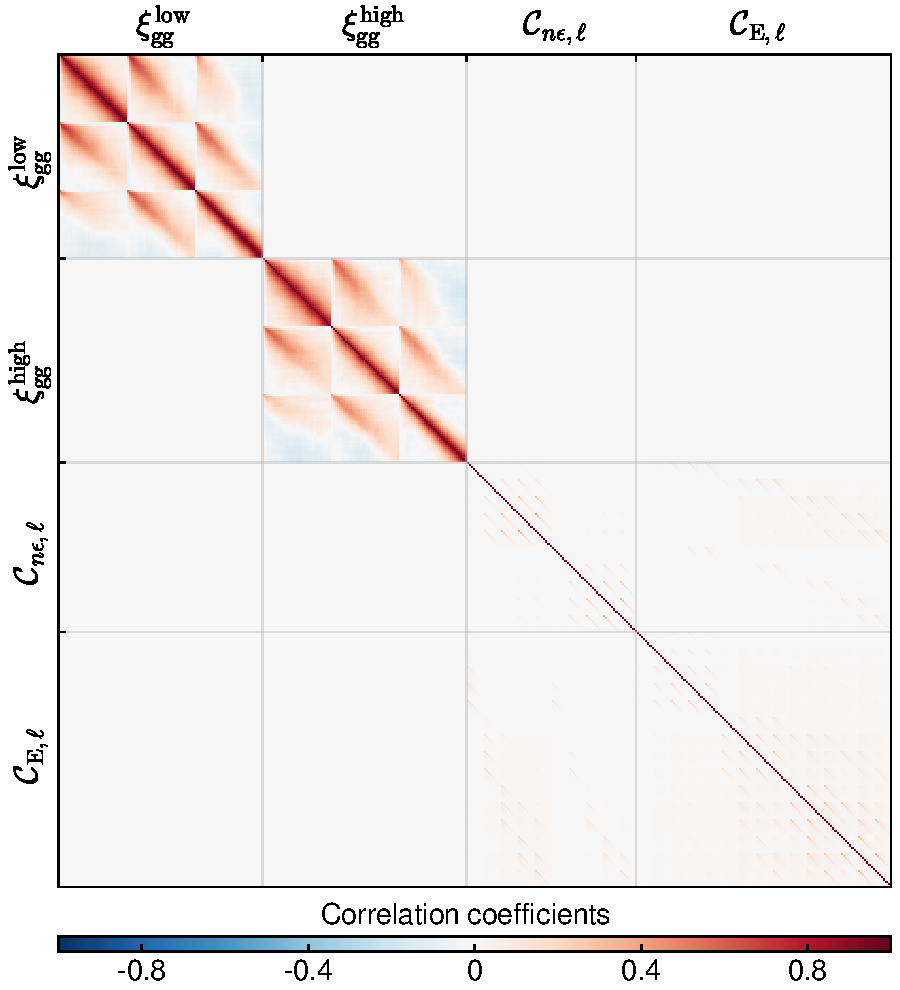
\includegraphics[width=\columnwidth]{Data_Plots/corr_paper_wedge+aPneE+aPeeE_obs_tot_theory}
		\caption{Correlation coefficients of the \tttp covariance matrix for the cosmic shear, $C_{\rm E}$, galaxy-galaxy lensing, $C_{n\epsilon}$ and galaxy clustering observables, $\xi_{\rm gg}$ (see Sect.~\ref{sec:data} for details).}
		\label{fig:ttttpcov}
	\end{center}
\end{figure}



\section{Parameter priors}
\label{app:priors}
This Appendix tabulates the adopted KiDS-1000 priors and sampling parameters in Table~\ref{tab:priors}.   
The uniform prior on the dimensionless Hubble constant, $h$, reflects distance-ladder $\pm 5 \sigma$ constraints from \citet{riess/etal:2016}, which encompasses the value of $h$ favoured by \citet{planck/etal:2018}.  
The uniform prior on the baryon density, $\omega_{\rm b}= \Omega_{\rm b}h^2$, reflects big bang nucleosynthesis $\pm 5 \sigma$ constraints from \citet{olive/etal:2014}.   
The uniform prior on the CDM density, $\omega_{\rm c} = \Omega_{\rm c}h^2$, reflects Supernova Type Ia $\pm 5 \sigma$ constraints on $\Omega_{\rm m}$ from \citet{scolnic/etal:2018} combined with the most extreme allowed values of $h$ and $\omega_{\rm b}$, given their priors.   

As discussed in Sect.~\ref{sec:KCAP} we choose to sample with an uninformative uniform prior on $S_8$ to avoid implicit informative priors from a uniform prior on the primordial power spectrum amplitude $A_{\rm s}$.    
We choose a fixed model for the properties of neutrinos, adopting the normal hierarchy at the minimum sum of masses, $\Sigma m_\nu = 0.06\,\mathrm{eV}$, following \citet{planck/etal:2018}.  
We consider extended models, including variations on neutrino mass in \citet{troester/etal:inprep}.

\begin{table}
\caption{KiDS-1000 sampling parameters and priors.}              % title of Table
\label{tab:priors}      % is used to refer this table in the text
\centering                                      % used for centering table
\begin{tabular}{lll}          % centered columns (4 columns)
\toprule
Parameter & Symbol & Prior \\    % table heading
\midrule                                   % inserts single horizontal line
Hubble constant & $h$ & $\bb{0.64,\,0.82}$ \\
Baryon density & $\omega_{\rm b}$ & $\bb{0.019,\,0.026}$ \\
CDM density & $\omega_{\rm c}$ & $\bb{0.051,\,0.255}$ \\
Density fluctuation amp. & $S_8$ & $\bb{0.1,\,1.3}$ \\
Scalar spectral index & $n_{\rm s}$ & $\bb{0.84,\,1.1}$ \\
\midrule
Linear galaxy bias & $b_1 \;[2]$ & $\bb{0.5,\,9}$ \\
Quadratic galaxy bias & $b_2 \;[2]$ & $\bb{-4,\,8}$ \\
Non-local galaxy bias & ${\gamma_3^-} \;[2]$ & $\bb{-8,\,8}$ \\
Virial velocity parameter & $a_{\rm vir} \;[2]$ & $\bb{0,\,12}$ \\
Intrinsic alignment amp. & $A_{\rm IA}$ & $\bb{-6,\,6}$ \\
Baryon feedback amp. & $A_{\rm baryon}$ & $\bb{2,\,3.13}$ \\
\midrule
Redshift offsets & ${\bf \delta_z}$ & ${\cal N}(\vek{\mu};\vek{C}_{\delta z})$ \\
\bottomrule
\end{tabular}
\tablefoot{Primary cosmological parameters for the flat $\Lambda$CDM model are listed in the first section. The second section lists astrophysical nuisance parameters to model galaxy bias (with independent parameters for each of the two BOSS redshift bins as indicated with the bracket $[2]$), intrinsic galaxy alignments, and baryon feedback.  Observational redshift nuisance parameters are listed in the final section. Prior values in square brackets are the limits of the adopted uniform top-hat priors.  ${\cal N}(\mu;C)$ corresponds to a five dimensional multivariate Gaussian prior with mean $\vek{\mu}$ and covariance $\vek{C}_{\delta z}$.}
\end{table}

The uniform prior on the scalar spectral index, $n_{\rm s}$, reflects a restriction in our likelihood implementation, where the \citet{sanchez/etal:2017} galaxy clustering likelihood becomes prohibitively slow for $n_{\rm s}>1.1$.  With the upper limit of the top-hat prior fixed by this computational limitation, we choose to symmetrise the prior around the theoretical expectation of $n_{\rm s}=0.97$.     In Fig.~\ref{fig:ns-prior} we demonstrate the impact of this informative prior on the BOSS-only galaxy clustering constraints, highlighting how informative this choice of prior is.   We argue that adopting an informative prior is justified however, given our theoretical prior knowledge of the Harrison-Zel'dovich spectrum.   Fig.~\ref{fig:ns-prior} also helps to illustrate that had we chosen an uninformative prior on $n_{\rm s}$ for our KiDS-1000-BOSS analysis, a decision taken more than a year before unblinding our analysis, this would have likely served to exacerbate any tension with the Planck CMB constraints. 

\begin{figure}
	\begin{center}
		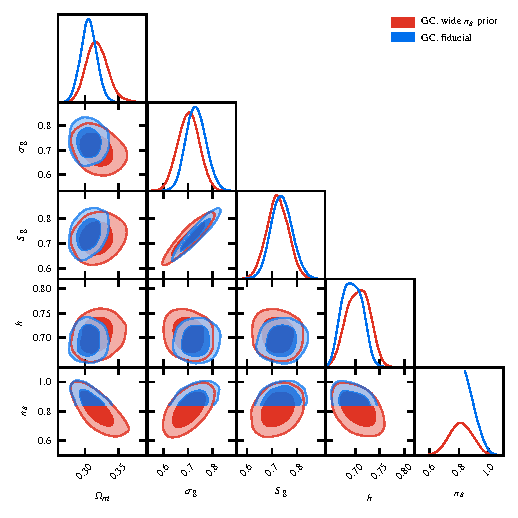
\includegraphics[width=\columnwidth]{Parameter_Plots/systematics/GC_ns_prior}
		\caption{The impact of the $n_{\rm s}$ prior: Comparing marginalised posterior distributions for the BOSS galaxy clustering analysis for our fiducial analysis (blue) with the constraints when adopting an uninformative prior on $n_{\rm s}$.   Opening the parameter space to arguably unphysical values of $n_{\rm s}$ favours lower values for $S_8$ and results in weaker constraints on $\Omega_{\rm m}$.}
		\label{fig:ns-prior}
	\end{center}
\end{figure}

Turning to astrophysical priors, the galaxy bias parameter top-hat priors on $b_1$, $b_2$,  $\gamma_3^-$, (Eq.~\ref{eq:pgg}), and on $a_{\rm vir}$ \citep[see the `fingers of god' model in equations 6 to 9 of][]{joachimi/etal:inprep},
match those adopted in \citet{troester/etal:2020}, which cover a wider range than those used in \citet{sanchez/etal:2017}.  
The two BOSS redshift slices have independent sets of parameters.   
Wide uniform priors for the intrinsic alignment parameter $A_{\rm IA}$ are chosen to be uninformative.    
Uniform priors on the baryon feedback parameter $A_{\rm baryon}$ are chosen such that the resulting \citet{mead/etal:2015} model of the non-linear matter power spectrum encompasses both the most aggressive feedback model from the \citet{vandaalen/etal:2011} suite of hydrodynamical simulations, along with the dark matter-only case where $A_{\rm baryon}=3.13$.

There are five additional correlated nuisance parameters, $\delta^i_z$, that model uncertainty in the mean of the source redshift distributions.  We adopt a multivariate Gaussian prior for the vector $\vek{\delta}_z$ with a mean $\vek{\mu} = (0.0001,0.0021,0.0129,0.0110,-0.0060)$, and a covariance, $C_{\delta z}$, as calibrated using mock galaxy catalogues in \citet{wright/etal:2020}.   
The diagonal terms of $\vek{C}_{\delta z}$ are typically at the level of $\sim(0.01)^2$, with off-diagonal correlation coefficients ranging between $~\sim 0.1$ and $\sim 0.3$ \citep[see section 3 and figure 2 of][for details]{hildebrandt/etal:inprep}.


\section{Parameter constraints}
\label{app:parameter-constraints}
This Appendix tabulates the maximum posterior (MAP) and marginalised constraints on the flat $\Lambda$CDM cosmological parameters, in Table~\ref{tab:fullparams}, for the different combinations of the three large-scale structure probes considered in this work.   For constraints from KiDS-1000 cosmic shear alone, we refer the reader to \citet{asgari/etal:inprep}.
\begin{landscape}
\begin{table}
\begin{center}
\caption{Parameter constraints for the probe combinations considered in this work: \tttp, cosmic shear (CS) and galaxy-galaxy lensing (GGL), cosmic shear and galaxy clustering (GC), and galaxy clustering by itself. 
We refer the reader to \citet{asgari/etal:inprep} for cosmic shear-only constraints. 
For each probe, the first column lists the MAP value with the PJ-HPD CI. 
If the PJ-HPD CI could not be robustly determined, no uncertainty estimate is provided. 
The second column for each probe lists the maximum of the marginal posterior, together with the marginal HPD CI. 
Parameter for which the marginal probability at either prior edge exceeds 13\% of the peak probability are deemed unconstrained and are denoted by a dash. 
Finally, parameters that are not sampled are left blank.
\label{tab:fullparams}}
\begin{tabular}{lllllllll}
    \toprule
    Parameter    & $3\times2$pt & $3\times2$pt& GC & GC& CS+GGL & CS+GGL& CS+GC & CS+GC \\ 
             & (joint) & (marginal)& (joint) & (marginal)& (joint) & (marginal)& (joint) & (marginal) \\ 

    \midrule
$S_8     $& $0.766^{+0.02}_{-0.014}$ & $0.765^{+0.017}_{-0.016}$& $0.762^{+0.054}_{-0.05}$ & $0.743^{+0.038}_{-0.05}$& $0.774^{+0.031}_{-0.029}$ & $0.761^{+0.024}_{-0.025}$& $0.766^{+0.018}_{-0.015}$ & $0.763^{+0.016}_{-0.016}$\\ [0.3 em]
$h^2\Omega_\mathrm{c}$& $0.123$ & $0.124^{+0.0096}_{-0.011}$& $0.136^{+0.0065}_{-0.018}$ & $0.123^{+0.011}_{-0.009}$& $0.0721^{+0.089}_{-0.016}$ & $0.12^{+0.057}_{-0.034}$& $0.126^{+0.0075}_{-0.013}$ & $0.124^{+0.01}_{-0.011}$\\ [0.3 em]
$h^2\Omega_\mathrm{b}$& $0.0225$ & --& $0.0246^{+0.0012}_{-0.0037}$ & --& $0.0258$ & --& $0.0219^{+0.0022}_{-0.0022}$ & --\\ [0.3 em]
$h       $& $0.695^{+0.03}_{-0.019}$ & $0.696^{+0.02}_{-0.026}$& $0.716^{+0.02}_{-0.035}$ & $0.687^{+0.029}_{-0.018}$& $0.642^{+0.1}_{-1.2e-05}$ & --& $0.695^{+0.022}_{-0.023}$ & $0.69^{+0.026}_{-0.02}$\\ [0.3 em]
$n_\mathrm{s}$& $0.901$ & --& $0.851^{+0.06}_{-0.01}$ & --& $0.947$ & --& $0.894^{+0.05}_{-0.042}$ & --\\ [0.3 em]
\midrule
$A_{\rm bary}$& $3.13^{+1.6e-05}_{-0.47}$ & --& $$ & & $3.13$ & --& $3.13$ & --\\ [0.3 em]
$A_{\rm IA}$& $1.07^{+0.27}_{-0.31}$ & $1.01^{+0.31}_{-0.28}$& $$ & & $0.974^{+0.32}_{-0.2}$ & $0.972^{+0.25}_{-0.26}$& $0.947^{+0.44}_{-0.31}$ & $0.892^{+0.35}_{-0.36}$\\ [0.3 em]
$\delta \bar{z_1}$& $1.93^{+11}_{-10}\times 10^{-3}$ & $2.8^{+8.8}_{-12}\times 10^{-3}$& $$ & & $1.41^{+8.4}_{-11}\times 10^{-3}$ & $2.15^{+8.7}_{-11}\times 10^{-3}$& $2.02^{+7.4}_{-14}\times 10^{-3}$ & $2.45^{+9.5}_{-12}\times 10^{-3}$\\ [0.3 em]
$\delta \bar{z_2}$& $0.0101^{+0.016}_{-0.0068}$ & $9.09^{+-9.1}_{-9.1}$& $$ & & $0.0102^{+0.014}_{-0.0069}$ & $8.75^{+-8.7}_{-8.8}$& $0.0117^{+0.013}_{-0.0085}$ & $0.0121^{+0.0095}_{-0.012}$\\ [0.3 em]
$\delta \bar{z_3}$& $-0.0207^{+0.0093}_{-0.01}$ & $-0.0204^{+0.01}_{-0.0093}$& $$ & & $-0.0206^{+0.0091}_{-0.0091}$ & $-0.0199^{+0.0092}_{-0.0092}$& $-0.013^{+0.0091}_{-0.012}$ & $-0.0119^{+0.0098}_{-0.011}$\\ [0.3 em]
$\delta \bar{z_4}$& $-0.0143^{+0.0076}_{-0.008}$ & $-0.0145^{+0.0082}_{-0.0076}$& $$ & & $-0.0138^{+0.0066}_{-0.0086}$ & $-0.012^{+0.0062}_{-0.009}$& $-0.0166^{+0.0098}_{-0.0064}$ & $-0.0156^{+0.0077}_{-0.0085}$\\ [0.3 em]
$\delta \bar{z_5}$& $5.23^{+8.3}_{-10}\times 10^{-3}$ & $4.54^{+10}_{-8.7}\times 10^{-3}$& $$ & & $6.06^{+7.3}_{-10}\times 10^{-3}$ & $6.85^{+8.7}_{-8.6}\times 10^{-3}$& $6.5^{+12}_{-7.1}\times 10^{-3}$ & $6.54^{+9.4}_{-9}\times 10^{-3}$\\ [0.3 em]
$b_1^{\rm lowz}$& $2^{+0.079}_{-0.083}$ & $2.04^{+0.064}_{-0.093}$& $2.01^{+0.13}_{-0.16}$ & $2.09^{+0.11}_{-0.13}$& $3.29^{+0.3}_{-0.81}$ & $3.14^{+0.55}_{-0.55}$& $1.99^{+0.09}_{-0.07}$ & $2.02^{+0.085}_{-0.07}$\\ [0.3 em]
$b_2^{\rm lowz}$& $0.3^{+0.62}_{-0.69}$ & $0.289^{+0.71}_{-0.61}$& $0.475^{+1.1}_{-0.83}$ & $0.624^{+0.96}_{-1}$& $0.968$ & --& $0.443^{+1}_{-0.67}$ & $0.326^{+1}_{-0.67}$\\ [0.3 em]
$\gamma_{3-}^{\rm lowz}$& $0.695^{+0.48}_{-0.54}$ & $0.879^{+0.44}_{-0.52}$& $0.688^{+0.59}_{-0.57}$ & $0.752^{+0.62}_{-0.56}$& $7.87$ & --& $0.594^{+0.58}_{-0.57}$ & $0.853^{+0.53}_{-0.52}$\\ [0.3 em]
$a_{\rm vir}^{\rm lowz}$& $4.14^{+0.84}_{-0.97}$ & $4.24^{+0.86}_{-0.96}$& $4.3^{+1.1}_{-1.2}$ & $4.44^{+1.1}_{-1.2}$& $$ & & $4.28^{+1.2}_{-1}$ & $4.37^{+1.1}_{-1.1}$\\ [0.3 em]
$b_1^{\rm highz}$& $2.13^{+0.095}_{-0.091}$ & $2.17^{+0.083}_{-0.093}$& $2.14^{+0.16}_{-0.16}$ & $2.23^{+0.13}_{-0.14}$& $2.3^{+0.33}_{-0.68}$ & $2.26^{+0.48}_{-0.52}$& $2.12^{+0.1}_{-0.094}$ & $2.17^{+0.092}_{-0.084}$\\ [0.3 em]
$b_2^{\rm highz}$& $-1.15^{+0.75}_{-0.41}$ & $-1.03^{+0.72}_{-0.46}$& $-0.948^{+2.3}_{-0.75}$ & $-0.901^{+2.3}_{-1}$& $5.82^{+2}_{-3.2}$ & --& $-1.16^{+1.8}_{-0.48}$ & $-0.951^{+1.7}_{-0.85}$\\ [0.3 em]
$\gamma_{3-}^{\rm highz}$& $0.369^{+0.8}_{-0.79}$ & $0.505^{+0.9}_{-0.62}$& $-0.126^{+0.94}_{-1.1}$ & $0.452^{+0.7}_{-1.2}$& $8^{+0.00058}_{-5.4}$ & --& $-0.0141^{+0.91}_{-0.91}$ & $0.412^{+0.8}_{-0.81}$\\ [0.3 em]
$a_{\rm vir}^{\rm highz}$& $1.18^{+1.5}_{-0.97}$ & --& $1.84^{+2.4}_{-1.8}$ & --& $$ & & $1.32^{+2.7}_{-1.3}$ & --\\ [0.3 em]
\midrule
$\Omega_\mathrm{m}$& $0.305^{+0.01}_{-0.015}$ & $0.306^{+0.012}_{-0.013}$& $0.313^{+0.0097}_{-0.017}$ & $0.307^{+0.011}_{-0.015}$& $0.239^{+0.11}_{-0.076}$ & $0.29^{+0.087}_{-0.07}$& $0.306^{+0.013}_{-0.012}$ & $0.307^{+0.012}_{-0.014}$\\ [0.3 em]
$\sigma_8$& $0.76^{+0.025}_{-0.02}$ & $0.759^{+0.02}_{-0.024}$& $0.75^{+0.045}_{-0.047}$ & $0.725^{+0.048}_{-0.036}$& $0.867^{+0.2}_{-0.17}$ & $0.729^{+0.13}_{-0.098}$& $0.758^{+0.028}_{-0.018}$ & $0.758^{+0.019}_{-0.024}$\\ [0.3 em]
$\sigma_{12}$& $0.743^{+0.03}_{-0.026}$ & $0.737^{+0.029}_{-0.027}$& $0.717^{+0.058}_{-0.035}$ & $0.707^{+0.046}_{-0.04}$& $0.887^{+0.15}_{-0.23}$ & $0.72^{+0.095}_{-0.14}$& $0.734$ & $0.732^{+0.03}_{-0.024}$\\ [0.3 em]
$S_{12}  $& $0.754^{+0.021}_{-0.013}$ & $0.754^{+0.015}_{-0.018}$& $0.751^{+0.038}_{-0.054}$ & $0.728^{+0.041}_{-0.045}$& $0.77^{+0.067}_{-0.046}$ & $0.757^{+0.036}_{-0.05}$& $0.753^{+0.022}_{-0.013}$ & $0.754^{+0.014}_{-0.019}$\\ [0.3 em]
$A_\mathrm{s}$& $1.85^{+0.25}_{-0.17}\times 10^{-9}$ & $1.79^{+0.22}_{-0.18}\times 10^{-9}$& $1.7^{+0.33}_{-0.16}\times 10^{-9}$ & $1.64^{+0.27}_{-0.18}\times 10^{-9}$& $5.34^{+5.2}_{-4.3}\times 10^{-9}$ & --& $1.81^{+0.27}_{-0.15}\times 10^{-9}$ & $1.78^{+0.21}_{-0.18}\times 10^{-9}$\\ [0.3 em]
$100\theta_{\rm MC}$& $1.05$ & $1.05^{+0.011}_{-0.015}$& $1.06^{+0.0082}_{-0.019}$ & $1.05^{+0.012}_{-0.013}$& $0.96^{+0.13}_{-0.023}$ & $1.09^{+0.039}_{-0.058}$& $1.05^{+0.009}_{-0.016}$ & $1.05^{+0.012}_{-0.014}$\\ [0.3 em]
    \bottomrule
\end{tabular}


\end{center}
\end{table}
\end{landscape}


\section{Sensitivity tests}
\label{app:sensitivity}
In this Appendix we present, with Fig.~\ref{fig:sensitivity_tests}, the marginalised posterior distributions for a selection of the \tttp sensitivity tests explored in Sect.~\ref{sec:results}.  
These tests were all shown to recover consistent constraints on $S_8$, in Fig.~\ref{fig:S8comp}, with the exception of the linear-only galaxy bias model analysis, as expected.    
Here we explore these tests in more detail.    

\begin{figure*}
	\begin{center}
		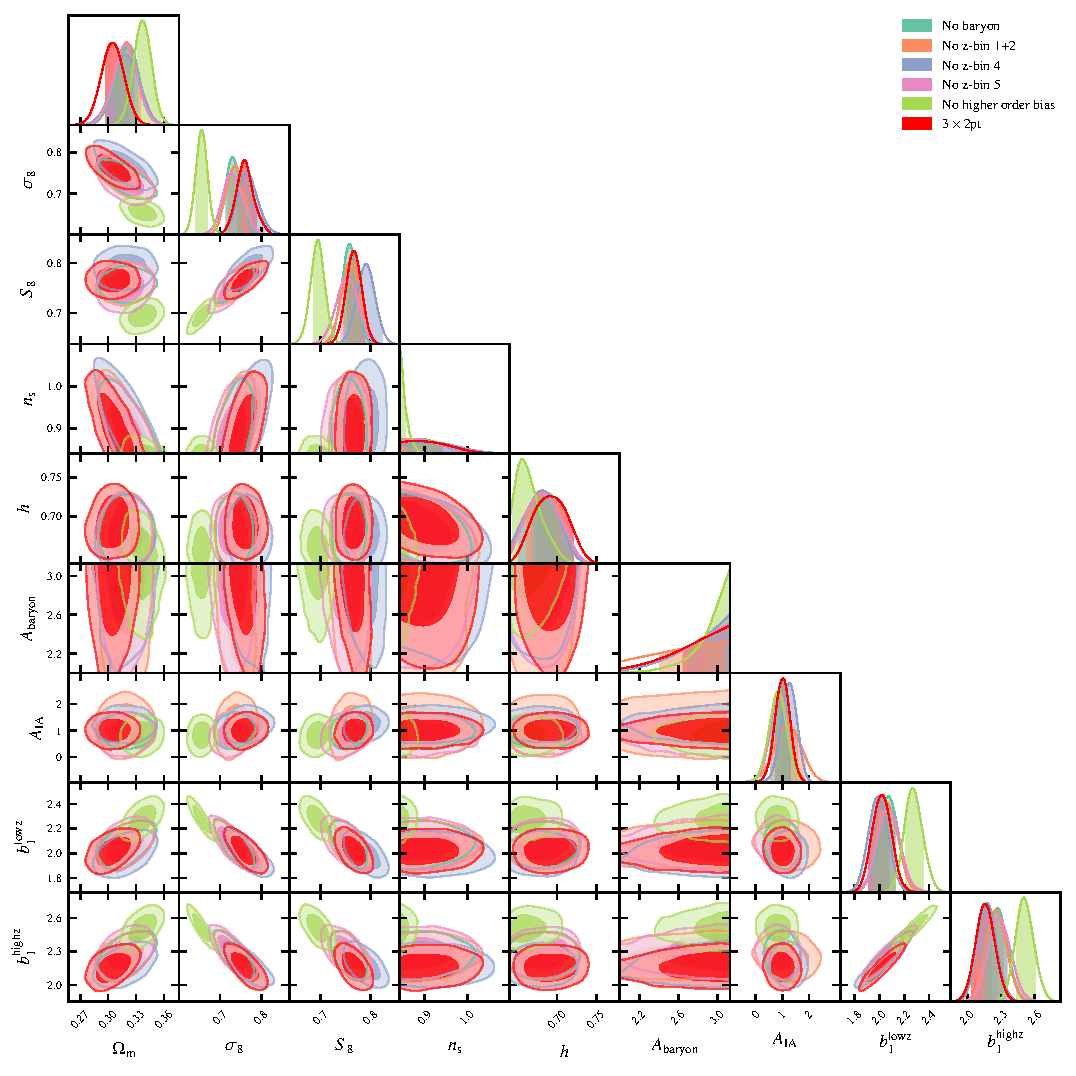
\includegraphics[width=\textwidth]{Parameter_Plots/systematics/blind_C_EE_nE_w_systematics_chains}
		\caption{Marginalised posterior distributions for the extended set of cosmological parameters shown in Fig.~\ref{fig:cosmology-params-all}, comparing the fiducial \tttp analysis (red) to a selection of our sensitivity test analyses where we ignore the impact of baryon feedback (the `No baryon' case, cyan), limit the analysis to a linear galaxy bias model (the `No higher order bias' case, green), and remove individual tomographic bins from our weak lensing observables (orange, purple and pink).}
		\label{fig:sensitivity_tests}
	\end{center}
\end{figure*}

We compare our analysis which fully marginalises over our uncertainty in the baryon feedback parameter (red), with our `No baryon' case (cyan), where $A_{\rm baryon}=3.13$, corresponding to the non-linear matter power spectrum for a dark-matter only cosmology.   
Here we find very little difference, as our \tttp analysis already favours high values of $A_{\rm baryon}$.   
Our choice of scales and adoption of the band-power cosmic shear statistic for this analysis also makes us less sensitive to uncertainties in the baryon feedback parameter, compared to a standard two-point correlation function analysis \citep{asgari/etal:2020_KD}.

The removal of the two highest photometric redshift bins (blue and purple) primarily impacts $S_8$.   
These two bins carry the majority of the signal-to-noise in our analysis, and so it is not surprising that the removal of nearly half the constraining data, in each case, can result in $\sim 1 \sigma$ changes in the recovered $S_8$.   
We refer the reader to \citet{asgari/etal:inprep} where we present a detailed internal consistency analysis of the cosmic shear signal, following \citet{kohlinger/etal:2019}, \citep[see also][]{efstathiou/lemos:2018},  concluding that the two highest photometric redshift bins are consistent with the full data set.   
A potential $\sim 2\sigma$-level flag is, however, raised in \citet{asgari/etal:inprep}, 
over the internal consistency of the second tomographic bin.  
In our analysis where we remove the two lowest photometric redshift bins (orange), we find that these bins contribute very little to the $S_8$ constraint, and only serve to tighten the constraints on the intrinsic alignment parameter $A_{\rm IA}$.

Finally we turn to the galaxy bias test (green), where we limit the analysis to a linear galaxy bias model, $b_1$, setting all higher-order bias terms in Eq. (\ref{eq:pgg}) to zero\footnote{Removing all higher-order galaxy bias terms also requires the uncoupling of $b_1$ from $\gamma_2$.}, as well as imposing a Gaussian galaxy velocity distribution by setting $a_{\rm vir}$ to zero.   
We can see that this induces a significant bias in the recovered constraints, as the amplitude of the linear galaxy bias increases in an attempt to model the enhanced power on small scales that the non-linear bias induces.   
The erroneous increase in $b_1$ leads to a significant decrease in the recovered $S_8$.  This result should serve as a point of caution for \tttp analyses that adopt an effective linear bias model \citep[see also the discussion in][]{asgari/etal:2020}, although we note that our analysis is particularly sensitive to the galaxy bias model given the high signal-to-noise BOSS clustering observations.


\section{Redundancy, pipeline validation and software review}
\label{app:codereview}

In this Appendix we briefly review the redundancy in the KiDS-1000 analysis, from pixels through to parameters.   Multi-band pixel processing and photometry in the optical has been carried out on the full KiDS-1000 data set using two independent pipelines, {\sc AstroWISE} and {\sc THELI} \citep{begeman/etal:2013, erben/etal:2013}.  This approach allowed us to resolve a range of different issues, primarily in the astrometric solution, for the handful of problem fields that resisted automated processing.  We adopt the {\sc AstroWISE} reduction for multi-band photometry and the {\sc THELI} $r$-band reduction for object detection and weak lensing shape measurement \citep{kuijken/etal:2019}.  We consider only one shape measurement technique, {\it lens}fit \citep{miller/etal:2013}, but this is calibrated using a series of different image simulations that vary the input galaxy properties to assess the sensitivity of the shear estimator to: the presence of blending with unresolved and undetected objects, blending due to enhanced galaxy clustering, photometric redshift selection bias, size-ellipticity correlations in the galaxy properties, varying stellar density, and the choice of smooth or realistic galaxy profiles \citep[see][for details]{kannawadi/etal:2019, giblin/etal:inprep}.  Our fiducial photometric redshift calibration has been compared to two additional independent calibration approaches, and has been validated on mock photometry catalogues \citep[see][for details]{wright/etal:2020, vandenbusch/etal:2020, hildebrandt/etal:inprep}.   Using a series of null-tests we have validated the resulting shear-redshift catalogues in \citet{giblin/etal:inprep}.    Our catalogue-to-observables pipeline, based on the two-point correlation function code {\sc TreeCorr} \citep{treecorr}, has been validated through an independent analysis using the alternative {\sc athena} package \citep{athena}, and through mock catalogue analysis \citep{joachimi/etal:inprep}.   Our cosmological inference code {\sc KCAP} with {\sc CAMB} \citep{lewis/etal:2000}, has been validated against the Core Cosmology Library \citep[CCL,][]{chisari/etal:2019} and through the recovery of input parameters in mock data analysis \citep{joachimi/etal:inprep}.  In \citet{asgari/etal:inprep} we also verify that we produce the same results in our cosmic-shear only analysis using a completely independent inference code based on {\sc MontePython} with {\sc CLASS} \citep{class, montepython, kohlinger/etal:2019,hildebrandt/etal:2020}.   Our analysis of BOSS follows \citet{sanchez/etal:2017}, which is in good agreement with the numerous independent parallel analyses of the same DR12 data set presented in \citet{alam/etal:2017}.


In regards to software review, we have adopted the `four-eye' approach, collaboratively building code through a git repository, with major updates reviewed through pull requests.   This approach has applied throughout the full pixels-to-parameters process, and to all types of software, both our significant tools, analysis code and, for the most part, simple paper support scripts.  On publication of this paper, our repositories will become open source for others to use and build upon, but with a caveat for users to recognise that we are not software engineers.   Adopting this style of software review for KiDS-1000 has been an extremely beneficial exercise for the team, with many lessons learnt for how to improve our software engineering skills and our approach to open source collaborative coding for future projects.     

\section{Post-unblinding analyses}
\label{app:unblinding}
This analysis was carried out `blind',  such that our final key result, our constraint on $S_8$, was unknown until all analysis choices were fixed.   Our blinding strategy creates three versions of the catalogue, where one is the truth, and the other two are modified to introduce up to a $\sim \pm 2\sigma$ deviation in the recovered value of $S_8$ \citep{kuijken/etal:2015, giblin/etal:inprep}.   In contrast to previous KiDS analyses, we set ourselves a challenge to only run our blind data analysis inference once, after fully developing and road-testing the pipeline using mock catalogues and data vectors \citep{joachimi/etal:inprep}.     Unexpectedly, the only analysis where we failed to meet this challenge were for data vectors that included galaxy clustering.   Here a bug in a naming convention in an updated {\sc CosmoSIS-CAMB} interface resulted in $\sim 0.5\sigma$ errors in the recovery of $\sigma_8$ in our initial BOSS re-analysis.  This was corrected and updated for our fiducial analysis before unblinding.

Our fiducial results, presented in Fig.~\ref{fig:cosmology-params} and tabulated in Appendix~\ref{app:parameter-constraints}, were carried out for all three blinds using a covariance matrix derived assuming a fiducial cosmology given by the best-fit parameters from \citet{troester/etal:2020}.  We reserved our iterated-covariance analysis, however, for post-unblinding, re-analysing the true data vector with an updated covariance matrix derived adopting the best-fit parameters from our initial blinded run of the true catalogue.   This iterative step changed our value for the full \tttp analysis $S_8$ by \ch{$X\sigma$}.   Our tension-consistency analysis with the CMB constraints from Planck was also conducted after unblinding, as we were unblind to Planck throughout the process.

As we are only interested in relative shifts in the sensitivity tests presented in Fig~\ref{fig:sensitivity_tests}, these were only conducted for a single blind, and re-calculated post-unblinding for the true catalogue.  Wishing to be fully transparent in this Appendix, we note that owing to limited resources the sensitivity test was not updated during the blinded phase of the project in order to correct for the {\sc CosmoSIS-CAMB} interface error which only impacted the BOSS constraints.   We argue that this was appropriate given the nature of the test and given that this error has been corrected post-unblinding.    Our cosmic shear and galaxy clustering analysis, featured in our internal consistency test in Fig.~\ref{fig:S8comp}, was also not re-processed blind after the BOSS error was corrected, as both our forecast in \citet{joachimi/etal:inprep}, and our initial analysis, confirmed that the constraints from our cosmic shear and galaxy clustering analysis were almost identical to constraints from the full \tttp analysis, which was correctly analysed for all three blinds.

As reported in \citet{giblin/etal:inprep}, co-author Kannawadi was unblinded early in the process to permit accurate calibration of the shear measurements in his re-analysis of KiDS-1000-like image simulations.   Co-authors Wright and Heymans also wish to record that they independently had a suspicion over which blind was the truth based on the changes that the SOM gold selection made to the blinded KiDS-1000 catalogue effective number density and ellipticity dispersion, compared to the impact the SOM selection made to the KiDS-VIKING-450 catalogue analysed in \citet{wright/etal:2020b}.  These suspicions were never shared with the rest of the team, nor discussed with each other, and on unblinding were found to both be false, and different!   This issue nevertheless highlighted to us the challenges of catalogue-level blinding for successive data releases where little has changed in the core data reduction process, if the people working at the coal-face of catalogue production are the same people working on the cosmological analysis.   Future KiDS blinding will therefore likely adopt the approach advocated by \citet{sellentin:2020}, where the covariance matrix is modified in the analysis.

\section{Expected $S_8$ differences between partially overlapping weak lensing surveys}
\label{app:expectedoffsets}
In this Appendix we construct a simple model to estimate the expected statistical fluctuation in $S_8$ constraints from partially overlapping weak lensing surveys, specifically our previous \citep[KV450,][]{wright/etal:2020b}, and our current KiDS analyses.

The $S_8$ measurement from KiDS-1000, $Z$, can be simplistically modelled as the area-weighted average of the measurement from the KV450 footprint, $X$, with the measurement from the additional area added for KIDS-1000, $Y$, as
\begin{equation}
  Z = \frac{A_X X + A_Y Y}{A_Z} \, ,
\end{equation}
where $A_X$ is the effective area of the KV450 footprint, $A_Z$ is the effective area of the KiDS-1000 footprint, and $A_Y = A_Z - A_X$, is the additional area added between the two data releases.  Approximating $X$ and $Y$ as uncorrelated disjoint areas, a significant approximation that ignores the large-scale correlations between them but is sufficient for this toy model, the uncertainty on $Z$, $\sigma_Z$, can be written as
\be
\sigma_Z^2 = \left(\frac{A_X}{A_Z}\right)^2 \sigma_X^2 + \left(\frac{A_Y}{A_Z}\right)^2 \sigma_Y^2
\label{eqn:sigmaZ}
\ee
where $\sigma_X$ and $\sigma_Y$ are the uncertainty on measurements $X$ and $Y$ respectively.   

Defining $\Delta = Z - X$, as the offset between the KiDS-1000 and KV450 measurements, we find \ch{being verbose here to work out why our results differ, won't include the next 2 equations in the paper}
\be
\Delta = X\, \left(\frac{A_X}{A_Z} -1 \right) + Y\, \frac{A_Y}{A_Z} \, ,
\ee
with an associated uncertainty
\be
\sigma_\Delta^2=\sigma_X^2\left(\frac{A_X}{A_Z} -1 \right)^2 + \sigma_Y^2\frac{A_Y^2}{A_Z^2} \, .
\ee
Substituting in $\sigma_Y$ from Eq.~(\ref{eqn:sigmaZ}) we find the uncertainty in terms of $\sigma_Z$ and $\sigma_X$ to be
\be
\sigma_\Delta^2 = \sigma_Z^2 + \sigma_X^2 - \frac{2A_X}{A_Z}\sigma_X^2 \, .
\ee

The absolute difference ($|\Delta|$) is distributed as a folded Gaussian, with mean $\mathrm{E}[|\Delta|] = \sqrt{2/\pi}\sigma_\Delta$, and cumulative distribution function, CDF of
\begin{equation}
   \mathrm{CDF}(x) = \mathrm{erf}\left(\frac{x}{\sigma_\Delta\sqrt{2}}\right) \,.
\end{equation}

Comparing the marginal $S_8$ constraints (M-HPD) from the two-point shear correlation function analysis of \citet[][KV450 X: $S_8 = 0.716^{+0.043}_{-0.038}$]{wright/etal:2020b} and \citet[][KiDS-1000 Z: $S_8=0.768^{+0.016}_{-0.020}$]{asgari/etal:inprep}, with the effective areas $A_{\rm KV450} = A_X = 341.3$ square degrees, and $A_{\rm KiDS-1000} = A_Z = 777.4$ square degrees, we find $|\Delta|=2.2\sigma_\Delta$, an offset that is expected to be found 2.5\% of the time.   Comparing the marginal $S_8$ constraints (M-HPD) from the $2\times2$pt analysis of \citet[][KV450+BOSS X: $S_8 = 0.728 \pm 0.026$]{troester/etal:2020} with the \tttp constraints from this analysis (KiDS-1000+BOSS Z: $S_8=0.766^{+0.018}_{-0.015}$), we find $|\Delta|=2.0\sigma_\Delta$, an offset that is expected to be found 4.5\% of the time.   

The probability of finding these offsets is low, but acceptable, particularly given that our conclusions significantly change when we compare the MAP with PJ-HPD constraints.  In this case from the two-point shear correlation function analysis of \citet[][KV450 X: $S_8 = 0.767^{+0.043}_{-0.038}$]{wright/etal:2020b} and \citet[][KiDS-1000 Z: $S_8=0.768^{+0.022}_{-0.015}$]{asgari/etal:inprep}, we find $|\Delta|=0.04\sigma_\Delta$, an offset that is expected to be found 97.5\% of the time.   This demonstrates that for an accurate assesment of the `tension' between results we need to consider the full shape of the posterior (see the discussion in Sect.~\ref{sec:planck_comp}).

This simple model analysis is sufficient to conclude that the increase in $S_8$ that we find between KV450 and KiDS-1000 is plausible, given statistical fluctuations.    A full assessment could be conducted by analysing a reasonable fraction of the 20,000 KiDS mock catalogues from \citet{joachimi/etal:inprep}, with the KiDS-1000 and KV450 footprints imposed.  Unfortunately this is, however, out-of-scope for this analysis, given the significant compute power that would be incurred.



\subsection{TT's original}

Let $X\sim N(0,\sigma^2)$, $Y\sim N(0,\sigma^2)$, and $Z=\frac{1}{2}(X+Y)$ with $Z\sim N(0, \frac{1}{2}\sigma^2)$. Think $X$=`KV450' and $Z$=`KiDS-1000'.

Now consider $\Delta=Z-X$, i.e., the difference between the `KiDS-1000' and `KV450'. We have $\Delta=\frac{1}{2}(Y-X)$, i.e., $\Delta\sim N(0, \frac{1}{2}\sigma^2)$.

The absolute difference ($|\Delta|$) is distributed as a folded Gaussian, with mean $\mathrm{E}[|\Delta|] = \sqrt{\frac{2}{\pi}}\sigma_\Delta = \sqrt{\frac{1}{\pi}}\sigma$, and CDF
\begin{equation}
   \mathrm{CDF}(x) = \mathrm{erf}\left(\frac{x}{\sigma_\Delta\sqrt{2}}\right) = \mathrm{erf}\left(\frac{x}{\sigma}\right) \ .
\end{equation}

Putting in numbers, the expected (absolute) offset between $X$ and $Z$ is $\approx 0.5\sigma$. There is a 16\% chance of getting offsets larger than $1\sigma$.

\paragraph{Improved treatment}
Since the m-calibration for KiDS-1000 is improved, the uncertainty of KiDS-1000 on the KV450 footprint is reduced. Furthermore, the footprint of KiDS-1000 is larger than twice the KV450 footprint. 
Let $\sigma_X$ be the KV450 uncertainty, $\sigma_Z$ the KiDS-1000 uncertainty, $A_X$ the area of the KV450 footprint, and $A_Z$ the area of the KiDS-1000 footprint. 
The KiDS-1000 measurement $Z$ is modelled as 
\begin{equation}
  Z = \frac{1}{A_Z}\left(A_X Y_1 + (A_Z-A_X) Y_2\right) \,
\end{equation}
the area-weighted average of the measurements of the KV450 footprint ($Y_1$ and the new area added for KiDS-1000 ($Y_2$). 
The joint measurements can be modelled as $(X, Y_1, Y_2)\sim N(0,\Sigma)$, where
\begin{equation}
  \Sigma = \begin{pmatrix}
              \sigma_X^2           & \sigma_X\sigma_{Y_1} & 0\\
              \sigma_X\sigma_{Y_1} & \sigma_{Y_1}^2       & 0\\
              0                    & 0                    & \sigma_{Y_2}^2
            \end{pmatrix}\, ,
\end{equation}
where $\sigma_{Y_1}=\sqrt{\frac{A_Z}{A_X}}\sigma_Z$ and $\sigma_{Y_2}=\sqrt{\frac{A_Z}{(A_Z-A_X)}}\sigma_Z$ are the uncertainties of the KiDS-1000 measurement on the KV450 and new footprint, respectively.  

\ch{I don't think this can be right though as here $\sigma_{Y_1} = \sigma_X$ and $\sigma_{Y_2} = \sigma_Y$ in my notation.  Putting these uncertainties into equation~\ref{eqn:sigmaZ}, you end up with $\sigma_Z^2 = \sigma_Z^2 + \sigma_Z^2$?}.


On the KV450 footprint the measurements $X$ and $Y_1$ are 100\% correlated. 
Now, let $\Delta = Z - X$, the offset between the KiDS-1000 and KV450 measurements. We have $\sigma_\Delta^2 = \mathrm{Var}[\Delta] = \sigma_X^2 + \sigma_Z^2 - 2\sqrt{\frac{A_X}{A_Z}}\sigma_X\sigma_Z$. The expectation and CDF for $|\Delta|$ follows as above.


\end{appendix}


%-------------------------------------------------------------------


\end{document}

